\documentclass[10pt,a4paper]{article}
\usepackage[margin=19mm]{geometry}
\usepackage{amsmath,amssymb,graphicx,array,hyperref}
\hypersetup{colorlinks=true,urlcolor=blue,linkcolor=blue}
\setlength{\parindent}{0pt}\setlength{\parskip}{6pt}
\newcommand{\rw}[1]{\mathord{#1\mkern2mu\wedge}}
\DeclareFontFamily{U}{articlebb}{}
\DeclareFontShape{U}{articlebb}{m}{n}{<-6> bbold5 <6-9> bbold7 <9-> bbold10}{}
\DeclareMathAlphabet{\matrixdigit}{U}{articlebb}{m}{n}
\pdfmapfile{+../../scaled-contact-article/fonts/blackboard/bbold.map}
\newcommand{\id}{\matrixdigit{1}}
\newcommand{\zmat}{\matrixdigit{0}}
\newcommand{\inertia}{\mathbb I}
\emergencystretch=2em
\begin{document}
\begin{center}
{\Large Measured inertia and sustained-contact repair}\\[5pt]
{\large Rigid-body collision model: verified progress and remaining gaps}\\
7 October 2026
\end{center}

\textbf{Result.} The 3D production adapter now accepts authoritative measured mass,
center of mass and inertia. A separate supported sphere/disk primitive includes
distinct static/dynamic friction and independent rolling/spin angular impulses.
It slows zero-slip rolling, arrests axial spin, and resolves transitions without
numerical reversal. No published restitution or friction value was changed or fitted.

\textbf{What this does not establish.} The supported primitive is not integrated
into the native general-impact/contact-group solver. The 24 glass comparisons
retain exactly their prior errors. No new improvement against experimental
measurements has been established, and a general authentic 2D/3D impact model
remains unqualified. The original symbolic article is preserved separately.

\section*{Diagnosis and implemented changes}
\begin{tabular}{p{.26\linewidth}p{.32\linewidth}p{.34\linewidth}}
\hline
Gap & Repair or evidence & Remaining scope\\\hline
Measured mass/COM/inertia rejected & Explicit SI mass-properties input; full tensor mapped to native principal axes & Source must supply real tensor; extent tests are necessary, not a realizability proof\\
No sustained rolling/spin resistance & Separate force and angular impulse channels; exact static/dynamic branches and arrest events & Scalar central inertia and one supported motion plane\\
Source density guard could be bypassed by new input & Profile checks authoritative mass and declared homogeneous-sphere inertia & Generic measured input is separate from source-specific assumptions\\
General directional static closure & Explicit rejection of partial arrest needing torque outside full $\hat{\boldsymbol s}/\hat{\boldsymbol n}$ span & Requires a specified physical zero/static-direction convention\\
Impact deformation/history & Previous local-memory and pressure-patch studies remain isolated & Opening, partial stick/slip, yield and group integration not repaired here\\\hline
\end{tabular}

\textbf{Input semantics.} Every measured override supplies mass, local COM, and a
symmetric body-axis inertia tensor about that COM. Collision geometry stays
geometric. Authored world position retains its COM meaning. Finite positive mass,
positive inertia eigenvalues, triangle inequalities and a geometry-extent bound
are checked. Three legacy scene preparations are bit-identical to revision
\texttt{512a1b2}. The documented glass profile retains its nominal density and
homogeneous-sphere assumption; it rejects contradictory overrides.

\textbf{Evidence classes.} Synthetic controls verify mechanics and numerical
implementation. Experimental residuals quantify source reproduction under fixed
inputs. Native timings measure a scoped kernel cost. These are distinct claims.
\newpage
\section*{Efficient calculation and the user's impulse notation}
With a fixed coordinate length $\ell$, combined momentum and velocity use
\[
\boldsymbol V=\begin{bmatrix}\boldsymbol v\\\ell\boldsymbol\omega\end{bmatrix},
\qquad \boldsymbol P=\begin{bmatrix}\boldsymbol p\\\boldsymbol L/\ell\end{bmatrix},
\qquad\mathbb M=\begin{bmatrix}m\id&\zmat\\\zmat&\inertia/\ell^2\end{bmatrix}.
\]
Small $\delta$ denotes physical contact impulses; $\Delta$ denotes body changes.
The components $\delta p_n,\delta p_t,\delta L_s,\delta L_n$ are scalars:
\[
\delta\boldsymbol p=\hat{\boldsymbol n}\,\delta p_n+
\hat{\boldsymbol t}\,\delta p_t,\qquad
\delta\boldsymbol L=\hat{\boldsymbol s}\,\delta L_s+
\hat{\boldsymbol n}\,\delta L_n,
\]
\[
\Delta\boldsymbol P=
\begin{bmatrix}\delta\boldsymbol p\\
\rw{\boldsymbol r}\,\delta\boldsymbol p/\ell+\delta\boldsymbol L/\ell
\end{bmatrix}.
\]
Here $\rw{\boldsymbol r}$ maps linear impulse to its lever moment in the
appropriate dimension; reversal is expressed through its transpose. In 3D,
the angular body change is the lever moment \emph{plus} the independent couple.
There is no linear $s$ component. In motion, $\hat{\boldsymbol t}$ is full
contact-relative velocity divided by its magnitude, and $\hat{\boldsymbol s}$
is full relative angular velocity divided by its magnitude.

For a supported sphere/disk define scalar translation $v$, rolling angular speed
$\omega_r$, radius $R$, scalar central inertia $I$, and slip $u=v-R\omega_r$.
Tangential force $f$ and independent rolling moment $M_r$ obey
\[
\begin{bmatrix}\dot u\\\dot\omega_r\end{bmatrix}=
\begin{bmatrix}F_d/m\\0\end{bmatrix}+
\begin{bmatrix}1/m+R^2/I&-R/I\\-R/I&1/I\end{bmatrix}
\begin{bmatrix}f\\M_r\end{bmatrix}.
\]
Only two coupled state derivatives are needed. Sliding uses
$f=-\mu_d N\operatorname{sign}u$; sticking solves $\dot u=0$ subject to
$|f|\le\mu_s N$. Rolling resistance has capacity
$|M_r|\le\mu_r a_rN$ and opposes nonzero rolling. At zero rolling, the holding
reaction is solved subject to this same capacity. Axial spin has declared
capacity $|M_n|\le\mu_n a_nN$ and is integrated only until its arrest.

Constant-branch accelerations are integrated exactly to the earliest arrest,
then constraints are re-evaluated. Physical moment lengths $a_r,a_n$ are separate
from coordinate length $\ell$. Normal/tangential restitution belong to impact
branches and are not reapplied in this persistent-load branch.

\textbf{3D qualification boundary.} Rotating this scalar-inertia branch produces
$\Delta\boldsymbol L=\rw{\boldsymbol r}\,\delta\boldsymbol p+
\delta\boldsymbol L$ with translating-support work included. It does not replace
$s$ by a rolling axis. At partial arrest, $s$ can be parallel to $n$ while a
transverse static moment is needed: the spatial wrapper explicitly rejects that
case. At complete zero motion, static constraint reactions are labeled rather
than inventing a velocity unit vector. The independent capacities are a declared
phenomenological law, not a measured coupled finite-patch friction budget.
\newpage
\section*{Mechanics controls: motion and spin}
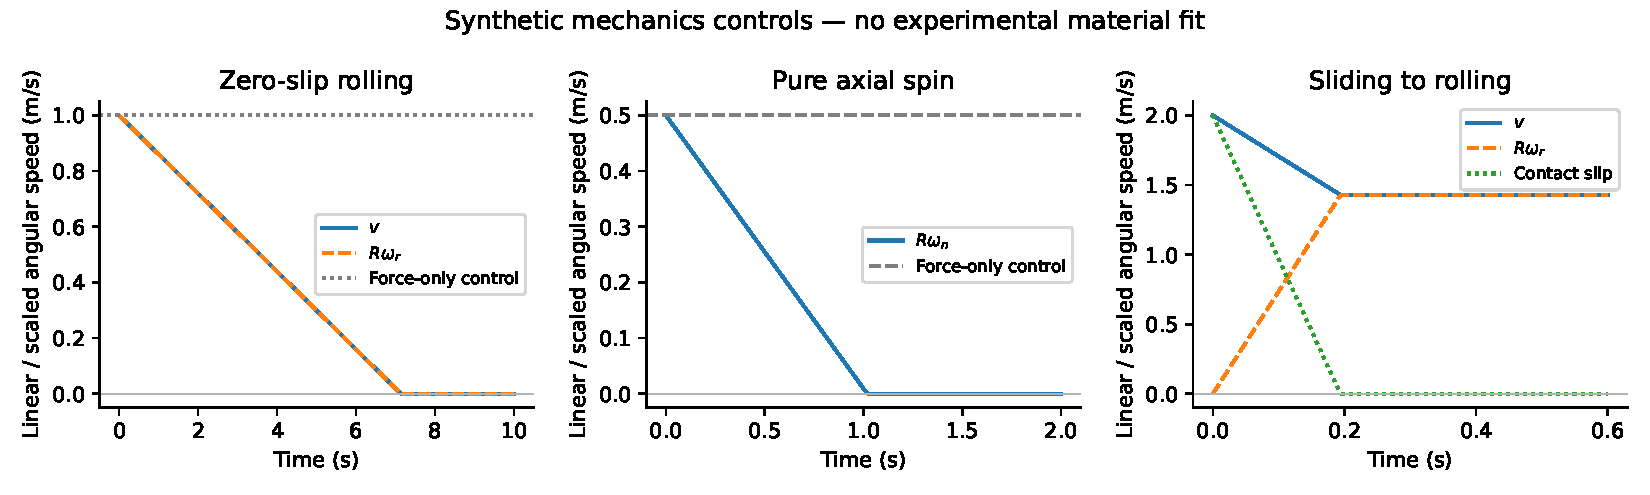
\includegraphics[width=\linewidth]{motion-controls.pdf}

All plot inputs below are synthetic verification fixtures. Dashed constant-speed
controls show why a force-only law at zero slip cannot dissipate rolling/spin.
They are not experimental comparisons or material calibration.

\begin{tabular}{llll}\hline
Input & Rolling control & Axial-spin control & Slide-to-roll control\\\hline
$m,R,I,N$ & \multicolumn{3}{l}{$1$ kg, $0.1$ m, $0.004$ kg m$^2$, $9.81$ N}\\
$v,\omega_r,\omega_n$ & $1,10,0$ & $0,0,5$ & $2,0,0$\\
$\mu_s,\mu_d$ & $0.5,0.3$ & $0.5,0.3$ & $0.8,0.3$\\
$\mu_r,a_r$ & $0.02,0.1$ m & $0,0$ & $0,0$\\
$\mu_n,a_n$ & $0,0$ & $0.1,0.02$ m & $0,0$\\\hline
\end{tabular}

\textbf{Checks.} Fifteen new tests pass, plus 24 existing regression tests. These
include static versus dynamic branches, zero-slip rolling, pure axial spin,
lever moment plus independent couple, moving-support work, tiny-motion preservation,
and explicit rejection of unsupported directional branches.

400 randomized controls pass energy and step-composition checks. Maximum relative
energy residual is \texttt{1.223e-15}; maximum scaled composition error is
\texttt{2.805e-16}. 100 rotated/moving-support controls have maximum
angular-impulse error \texttt{2.010e-15} N m s. These are finite test samples,
not a general error theorem or proof of experimental authenticity.

\textbf{Native inertia dynamics.} A free asymmetric-body rotation test initially
missed its $10^{-7}$ momentum-error tolerance at 64 steps: relative error
$3.29\cdot10^{-7}$. Refinement to 256 steps gives $8.24\cdot10^{-8}$ and passes
the unchanged gate. The retained refinement shows first-order gyroscopic
integration convergence; no output or material parameter was fitted.

\textbf{Energy ledger.} The supported result records sliding, rolling and axial
spin losses separately. For a translating plane with velocity $\boldsymbol U$,
support work is $\boldsymbol U^T\delta\boldsymbol p$. Body energy change equals
drive work plus support work minus these losses. The new API returns both
relative and world energy, preventing a moving support from being mislabeled
as contact dissipation.
\newpage
\section*{Comparison to experimental reality}
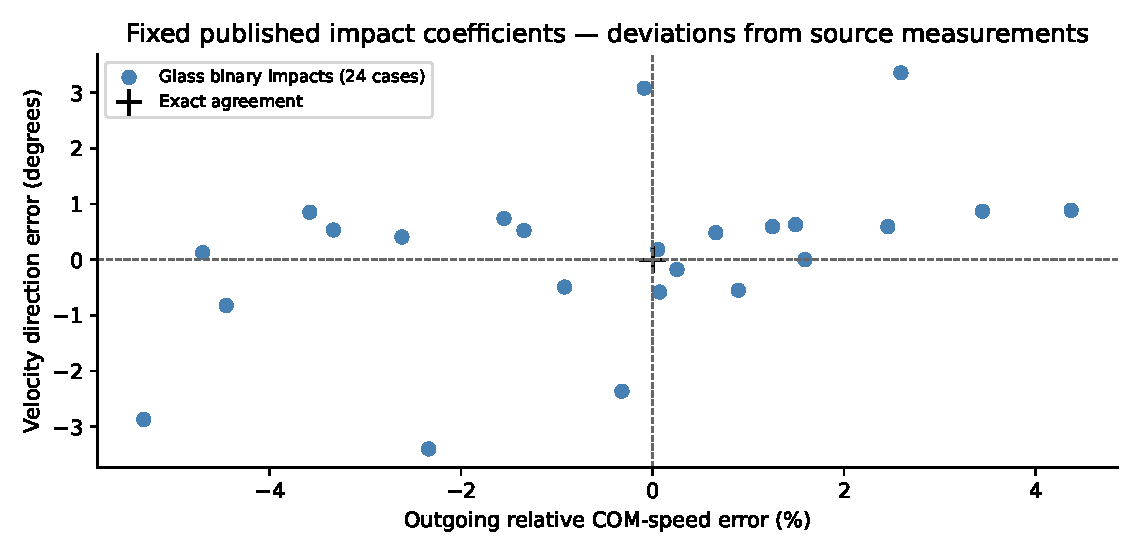
\includegraphics[width=\linewidth]{glass-deviation.pdf}

The diagram maps each outgoing \emph{relative COM velocity} to magnitude and
direction error for the same incoming worksheet state. The origin is exact
agreement. Only one collision family is plotted; no angular-velocity accuracy
is implied because the worksheet spin is reconstructed, not independently measured.

\begin{tabular}{p{.34\linewidth}p{.23\linewidth}p{.34\linewidth}}\hline
24 glass binary impacts & Current result & Comparison status\\\hline
Normal-speed RMSE & 0.036674 m/s & Unchanged from prior comparison\\
COM-tangent-speed RMSE & 0.017805 m/s & Unchanged; source reconstruction retained\\
Joint input-normalized RMSE & 0.024156 & Unchanged; dimensionless component RMS\\
Native analytic/energy checks & 24/24 & Numerical mechanics checks only\\\hline
\end{tabular}

\begin{tabular}{ll}\hline
Fixed published impact inputs & Value\\\hline
Normal restitution $e_n$ & 0.97\\
Tangential restitution $e_t$ & 0.44\\
Pair sliding friction & 0.092\\\hline
\end{tabular}

The Cornell worksheet and coefficient chart may share characterization trials;
this is source reproduction, not an independently calibrated held-out validation.
Nominal diameter and homogeneous inertia are source assumptions. Separate
static/dynamic/rolling/spin parameters and independent measured spin are absent.
Consequently this replay checks compatibility of the native adapter, not the new
supported resistance law. All original per-case states and residuals are retained.

Other public-data results remain unchanged: GAUGE sliding forecasts have
6.962/10.824/2.880 mm position RMSE for wood/plastic/metal; its conditional
bounce normal-speed RMSE is 0.381 m/s with substantial timing sensitivity. The
134 unique limestone first-rocking ratios have a geometry-only comparator RMSE
0.0390. MIT's 1,718 signed planar states and GAUGE's 160 spatial impact trials
are imports/diagnostics, not newly qualified endpoint predictions. These metrics
have different units and protocols and must not be pooled into an accuracy score.
\newpage
\section*{Native cost, practical limits and next model work}
The warning-free C++17 kernel uses fifteen SoA input arrays and eleven response
arrays indexed by body $k$. It matches all 400 Python fixtures; maximum scaled
output difference is zero on this compiler. No fast-math option is used.

\begin{tabular}{rrrr}\hline
Independent updates & ns/update median & Total ms & Array MB\\\hline
100 & 48.60 & 0.005 & 0.02 \\
10,000 & 46.94 & 0.469 & 2.08 \\
100,000 & 80.94 & 8.094 & 20.80 \\
1,000,000 & 81.41 & 81.406 & 208.00 \\
\hline\end{tabular}

Five timed repetitions follow one warmup. Input loads, all output stores,
branch and energy checks are included. Allocation, collision detection,
pose/quaternion evolution, changing normal load, impacts and contact-group solving
are excluded. Larger arrays change the memory working set. Repeated independent
fixtures are not a million-body interacting simulation. No baseline speedup or
2$\times$ gate is claimed. Flat indices and explicit load/store channels are
suitable for a later Vektor Flow port; no port or GPU result is claimed here.

\textbf{What is still missing.} General zero/static-direction closure, contact
opening and pressure evolution, partial sticking/sliding with shear history,
elastic mode energy and appropriate material yield are not captured by this
constant-load branch. Arbitrary full-inertia bodies and simultaneous contact
groups also remain separate integration tasks. Static/dynamic and angular
capacities must eventually be tied to independently characterized contact physics,
not just bounded separately because that is easy to implement.

\textbf{Best next extension.} Keep rigid bodies but add a small local contact
state for shear displacement and elastic/mode energy, with unilateral normal
opening, release of stored energy, static/dynamic transitions, finite-patch
force/couple budgets and an auditable work ledger. Start on a single measured
oblique impact, then require held-out improvement under fixed published inputs
before integrating the branch into general contact groups. The existing patch
and memory studies provide components, not a completed constitutive closure.

Maw--Barber--Fawcett's oblique elastic-sphere analysis supports investigating
tangential compliance and partial stick/slip. It does not supply every parameter
for rocks or rubber, nor validate this supported-contact primitive. Independently
measured mass/inertia, contact timing, endpoint spin, pair-specific friction and
contact stiffness/dissipation remain priorities for stronger prediction tests.

\textbf{Sources and reproduction.}
\begin{itemize}
\item Cornell original glass \href{https://grainflowresearch.mae.cornell.edu/impact/data/Results-3mmglass-binary}{worksheet} and \href{https://grainflowresearch.mae.cornell.edu/impact/data/Impact%20Results.html}{coefficient catalog}; worksheet SHA-256 in replay summary.
\item Maw, Barber, Fawcett (1976), \emph{The oblique impact of elastic spheres}, Wear 38, 101--114. \href{https://websites.umich.edu/~jbarber/Wear1976.pdf}{Author-hosted paper}, DOI 10.1016/0043-1648(76)90201-5.
\item Previous public datasets, protocols, uncertainty and hashes:\\repository \texttt{research/public-validation-data/README.md} and its report.
\item Current evidence/code: \texttt{research/contact-gap-fix/}; README gives test, audit, replay, benchmark and report commands. Temporary archive relocation is recorded separately; no measurement was deleted.
\end{itemize}
\end{document}
